\documentclass[tikz,border=0pt]{standalone}
\usetikzlibrary{calc}

\begin{document}
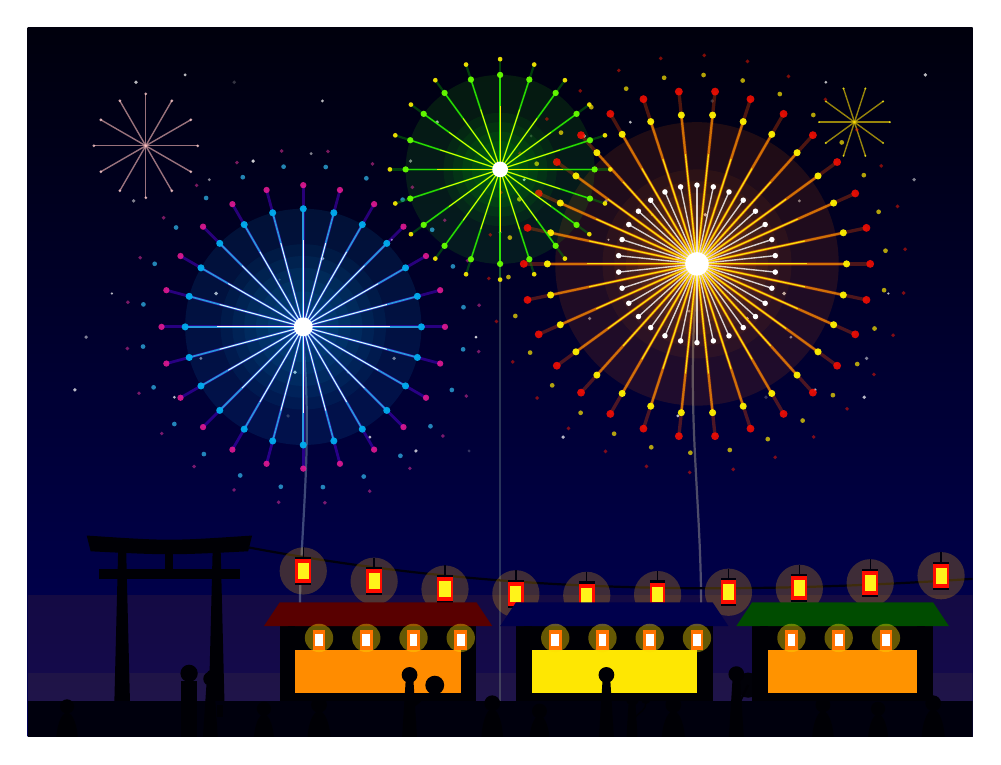
\begin{tikzpicture}
  % Clip to canvas size (12cm x 9cm, 4:3 ratio)
  \clip (0,0) rectangle (12,9);

  % Deep night sky gradient
  \fill[top color=black!95!blue, bottom color=blue!35!black] (0,-0.1) rectangle (12,9);

  % Scattered stars (using deterministic math to avoid seed issues)
  \foreach \x in {1,2,...,11} {
    \foreach \y in {4,5,6,7,8} {
      \pgfmathsetmacro{\xoff}{0.4*sin(\x*70 + \y*50)}
      \pgfmathsetmacro{\yoff}{0.4*cos(\x*40 + \y*80)}
      \pgfmathsetmacro{\staropacity}{0.2 + 0.6*abs(sin(\x*120 + \y*90))}
      \pgfmathsetmacro{\starsize}{0.015 + 0.01*abs(cos(\x*90 + \y*120))}
      \fill[white, opacity=\staropacity] (\x+\xoff, \y+\yoff) circle (\starsize);
    }
  }

  % Distant glowing background circles for fireworks
  \fill[orange!80!red, opacity=0.12] (8.5, 6) circle (1.8);
  \fill[cyan!80!blue, opacity=0.12] (3.5, 5.2) circle (1.5);
  \fill[green!80!yellow, opacity=0.1] (6, 7.2) circle (1.2);

  % Trails of ascending fireworks
  \draw[white!80!yellow, line width=0.8pt, opacity=0.3, line cap=round] (8.5,0.4) to[out=85,in=-95] (8.5,5.8);
  \draw[white!80!cyan, line width=0.8pt, opacity=0.3, line cap=round] (3.5,0.4) to[out=95,in=-85] (3.5,5.0);
  \draw[white!80!green, line width=0.6pt, opacity=0.2, line cap=round] (6.0,0.4) to[out=90,in=-90] (6.0,7.0);

  % Distant Firework 1 (Pink)
  \begin{scope}[shift={(1.5,7.5)}, scale=0.55]
    \foreach \a in {0,30,...,330} {
      \draw[pink, line width=0.5pt, opacity=0.6] (0,0) -- (\a:1.2);
      \fill[pink!80!white, opacity=0.8] (\a:1.2) circle (0.035);
    }
  \end{scope}
  
  % Distant Firework 2 (Gold/Yellow)
  \begin{scope}[shift={(10.5,7.8)}, scale=0.45]
    \foreach \a in {0,36,...,324} {
      \draw[yellow!80!orange, line width=0.5pt, opacity=0.6] (0,0) -- (\a:1.0);
      \fill[yellow!90!white, opacity=0.8] (\a:1.0) circle (0.03);
    }
  \end{scope}

  % Main Firework 1 (Orange/Red/Yellow - Right)
  \begin{scope}[shift={(8.5,6)}]
    % Inner glow
    \foreach \r in {1,2,...,8} {
      \fill[orange, opacity=0.06] (0,0) circle (\r*0.15);
    }
    % Rays
    \foreach \a in {0,12,...,348} {
      \draw[red!40!orange, line width=1.2pt, opacity=0.3] (0,0) -- (\a:2.2);
      \draw[orange!85!yellow, line width=0.8pt, opacity=0.7] (0,0) -- (\a:1.9);
      \draw[yellow!95!white, line width=0.4pt, opacity=0.9] (0,0) -- (\a:1.4);
      \fill[yellow, opacity=0.95] (\a:1.9) circle (0.045);
      \fill[red!90!orange, opacity=0.85] (\a:2.2) circle (0.05);
    }
    % Outer detached sparks
    \foreach \a in {4,16,...,352} {
      \fill[yellow!90!orange, opacity=0.7] (\a:2.4) circle (0.03);
      \fill[red!80!orange, opacity=0.5] (\a:2.65) circle (0.025);
    }
    % Inner ring of white sparks
    \foreach \a in {6,18,...,354} {
      \draw[white, line width=0.5pt, opacity=0.8] (0,0) -- (\a:1.0);
      \fill[white] (\a:1.0) circle (0.035);
    }
    \fill[white] (0,0) circle (0.15);
  \end{scope}

  % Main Firework 2 (Cyan/Blue/Magenta - Left)
  \begin{scope}[shift={(3.5,5.2)}]
    % Inner glow
    \foreach \r in {1,2,...,7} {
      \fill[cyan, opacity=0.06] (0,0) circle (\r*0.15);
    }
    % Rays
    \foreach \a in {0,15,...,345} {
      \draw[blue!60!magenta, line width=1.0pt, opacity=0.4] (0,0) -- (\a:1.8);
      \draw[cyan!85!white, line width=0.6pt, opacity=0.8] (0,0) -- (\a:1.5);
      \draw[white, line width=0.3pt, opacity=0.95] (0,0) -- (\a:1.1);
      \fill[cyan, opacity=0.95] (\a:1.5) circle (0.045);
      \fill[magenta!90!white, opacity=0.85] (\a:1.8) circle (0.04);
    }
    % Outer detached sparks
    \foreach \a in {7,22,...,352} {
      \fill[cyan!80!white, opacity=0.7] (\a:2.05) circle (0.03);
      \fill[magenta!80!white, opacity=0.5] (\a:2.25) circle (0.025);
    }
    \fill[white] (0,0) circle (0.12);
  \end{scope}

  % Main Firework 3 (Green/Yellow - Center Top)
  \begin{scope}[shift={(6,7.2)}]
    % Inner glow
    \foreach \r in {1,2,...,6} {
      \fill[green, opacity=0.06] (0,0) circle (\r*0.12);
    }
    % Rays
    \foreach \a in {0,18,...,342} {
      \draw[green!60!black, line width=0.8pt, opacity=0.4] (0,0) -- (\a:1.4);
      \draw[green!80!yellow, line width=0.5pt, opacity=0.8] (0,0) -- (\a:1.2);
      \draw[yellow, line width=0.3pt, opacity=0.95] (0,0) -- (\a:0.8);
      \fill[green!60!yellow, opacity=0.95] (\a:1.2) circle (0.04);
      \fill[yellow, opacity=0.9] (\a:1.4) circle (0.03);
    }
    \fill[white] (0,0) circle (0.1);
  \end{scope}

  % Soft illumination on the ground/stalls from the fireworks
  \fill[orange, opacity=0.08] (0,0) rectangle (12,1.8);
  \fill[yellow!80!orange, opacity=0.05] (0,0) rectangle (12,0.8);

  % Torii Gate Silhouette (Left Foreground)
  \begin{scope}[shift={(0.8, 0.4)}]
    % Pillars
    \fill[black!98!blue] (0.3, 0) -- (0.35, 2.0) -- (0.45, 2.0) -- (0.5, 0) -- cycle;
    \fill[black!98!blue] (1.5, 0) -- (1.55, 2.0) -- (1.65, 2.0) -- (1.7, 0) -- cycle;
    % Lower beam (Nuki)
    \fill[black!98!blue] (0.1, 1.60) rectangle (1.9, 1.72);
    % Top beam (Kasagi & Shimagi)
    \fill[black!98!blue] (0.0, 1.95) .. controls (1.0, 1.90) .. (2.0, 1.95) -- (2.05, 2.15) .. controls (1.0, 2.08) .. (-0.05, 2.15) -- cycle;
    % Gakuzuka (center support)
    \fill[black!98!blue] (0.95, 1.60) rectangle (1.05, 1.98);
  \end{scope}

  % Rope for Hanging Festival Lanterns (Chouchin)
  \draw[black!95!blue, line width=0.8pt] (2.8, 2.4) .. controls (6, 1.8) and (9, 1.8) .. (12, 2.0);
  
  % Hanging Lanterns along the rope
  \foreach \lx/\ly in {3.5/2.25, 4.4/2.12, 5.3/2.02, 6.2/1.96, 7.1/1.94, 8.0/1.95, 8.9/1.98, 9.8/2.03, 10.7/2.10, 11.6/2.19} {
    % Lantern glow
    \fill[yellow!40!orange, opacity=0.25] (\lx, \ly-0.15) circle (0.3);
    % Lantern body
    \fill[red!90!orange] (\lx-0.1, \ly-0.3) rectangle (\lx+0.1, \ly);
    \fill[yellow!90!white] (\lx-0.07, \ly-0.25) rectangle (\lx+0.07, \ly-0.05);
    % Top and bottom caps
    \fill[black!95!blue] (\lx-0.1, \ly) rectangle (\lx+0.1, \ly+0.03);
    \fill[black!95!blue] (\lx-0.1, \ly-0.33) rectangle (\lx+0.1, \ly-0.3);
    % Hanging string
    \draw[black!95!blue, line width=0.5pt] (\lx, \ly) -- (\lx, \ly+0.15);
  }

  % Food Stalls (Yatai)
  % Stall 1 (Left - Red Roof)
  \fill[black!98!blue] (3.2,0.4) rectangle (5.7,1.4);
  \fill[red!35!black] (3.0,1.4) -- (3.2,1.7) -- (5.7,1.7) -- (5.9,1.4) -- cycle;
  \fill[orange!90!yellow] (3.4,0.5) rectangle (5.5,1.1); % interior warm light
  \fill[black!98!blue] (3.3,0) rectangle (3.4,1.4);
  \fill[black!98!blue] (5.5,0) rectangle (5.6,1.4);
  \fill[black!98!blue] (3.3,0.4) rectangle (5.6,0.55);
  % Stall 1 Hanging Lanterns
  \foreach \lx in {3.7, 4.3, 4.9, 5.5} {
    \fill[yellow!80!orange, opacity=0.4] (\lx, 1.25) circle (0.18);
    \fill[orange!90!red] (\lx-0.08, 1.1) rectangle (\lx+0.08, 1.35);
    \fill[white] (\lx-0.05, 1.15) rectangle (\lx+0.05, 1.3);
  }

  % Stall 2 (Middle - Blue Roof)
  \fill[black!98!blue] (6.2,0.4) rectangle (8.7,1.4);
  \fill[blue!30!black] (6.0,1.4) -- (6.2,1.7) -- (8.7,1.7) -- (8.9,1.4) -- cycle;
  \fill[yellow!90!orange] (6.4,0.5) rectangle (8.5,1.1); % interior warm light
  \fill[black!98!blue] (6.3,0) rectangle (6.4,1.4);
  \fill[black!98!blue] (8.5,0) rectangle (8.6,1.4);
  \fill[black!98!blue] (6.3,0.4) rectangle (8.6,0.55);
  % Stall 2 Hanging Lanterns
  \foreach \lx in {6.7, 7.3, 7.9, 8.5} {
    \fill[yellow!80!orange, opacity=0.4] (\lx, 1.25) circle (0.18);
    \fill[orange!90!red] (\lx-0.08, 1.1) rectangle (\lx+0.08, 1.35);
    \fill[white] (\lx-0.05, 1.15) rectangle (\lx+0.05, 1.3);
  }

  % Stall 3 (Right - Green Roof)
  \fill[black!98!blue] (9.2,0.4) rectangle (11.5,1.4);
  \fill[green!30!black] (9.0,1.4) -- (9.2,1.7) -- (11.5,1.7) -- (11.7,1.4) -- cycle;
  \fill[orange!85!yellow] (9.4,0.5) rectangle (11.3,1.1); % interior warm light
  \fill[black!98!blue] (9.3,0) rectangle (9.4,1.4);
  \fill[black!98!blue] (11.3,0) rectangle (11.4,1.4);
  \fill[black!98!blue] (9.3,0.4) rectangle (11.4,0.55);
  % Stall 3 Hanging Lanterns
  \foreach \lx in {9.7, 10.3, 10.9} {
    \fill[yellow!80!orange, opacity=0.4] (\lx, 1.25) circle (0.18);
    \fill[orange!90!red] (\lx-0.08, 1.1) rectangle (\lx+0.08, 1.35);
    \fill[white] (\lx-0.05, 1.15) rectangle (\lx+0.05, 1.3);
  }

  % Ground Silhouette
  \fill[black!95!blue] (0,-0.1) rectangle (12,0.45);

  % People's Silhouettes (Wearing Yukata and holding accessories)
  % Couple 1 (Left - Woman with hair bun and obi, man)
  \fill[black!98!blue] (1.95,-0.1) -- (1.95,0.7) -- (2.15,0.7) -- (2.15,-0.1) -- cycle; % Man body
  \fill[black!98!blue] (2.05,0.8) circle (0.11); % Man head
  \fill[black!98!blue] (2.22,-0.1) -- (2.27,0.65) -- (2.37,0.65) -- (2.42,-0.1) -- cycle; % Woman body
  \fill[black!98!blue] (2.32,0.73) circle (0.09); % Woman head
  \fill[black!98!blue] (2.32,0.80) circle (0.04); % Hair bun
  \fill[black!98!blue] (2.40, 0.25) rectangle (2.48, 0.4); % Obi bow

  % Person holding Uchiwa (Japanese round fan)
  \fill[black!98!blue] (4.75,-0.1) -- (4.80,0.7) -- (4.90,0.7) -- (4.95,-0.1) -- cycle;
  \fill[black!98!blue] (4.85,0.78) circle (0.1);
  \draw[black!98!blue, line width=1.5pt] (4.90, 0.4) to[out=30, in=120] (5.10, 0.5); % arm
  \draw[black!98!blue, line width=0.8pt] (5.10, 0.5) -- (5.17, 0.65); % fan stick
  \fill[black!98!blue] (5.17, 0.65) circle (0.12); % fan shape

  % Parent and Child (Child holding a water balloon)
  \fill[black!98!blue] (7.25,-0.1) -- (7.30,0.7) -- (7.40,0.7) -- (7.45,-0.1) -- cycle; % Parent body
  \fill[black!98!blue] (7.35,0.78) circle (0.1); % Parent head
  \fill[black!98!blue] (7.60,-0.1) -- (7.63,0.4) -- (7.72,0.4) -- (7.75,-0.1) -- cycle; % Child body
  \fill[black!98!blue] (7.68,0.47) circle (0.08); % Child head
  \draw[black!98!blue, line width=0.5pt] (7.72, 0.25) to[out=45, in=-90] (7.85, 0.42); % string
  \fill[black!98!blue] (7.85, 0.47) circle (0.06); % balloon

  % Person holding Cotton Candy (Wata-ame)
  \fill[black!98!blue] (8.90,-0.1) -- (8.95,0.7) -- (9.05,0.7) -- (9.10,-0.1) -- cycle;
  \fill[black!98!blue] (9.00,0.79) circle (0.1);
  \draw[black!98!blue, line width=0.8pt] (9.05, 0.45) -- (9.15, 0.65); % stick
  \fill[black!98!blue, opacity=0.95] (9.15, 0.65) circle (0.16); % cotton candy puff

  % Other background silhouettes to populate the festival
  \fill[black!98!blue] (0.5,-0.1) ellipse (0.14 and 0.4);
  \fill[black!98!blue] (0.5,0.38) circle (0.09);
  
  \fill[black!98!blue] (3.0,-0.1) ellipse (0.13 and 0.38);
  \fill[black!98!blue] (3.0,0.35) circle (0.09);

  \fill[black!98!blue] (3.7,-0.1) ellipse (0.15 and 0.42);
  \fill[black!98!blue] (3.7,0.4) circle (0.1);

  \fill[black!98!blue] (5.9,-0.1) ellipse (0.14 and 0.45);
  \fill[black!98!blue] (5.9,0.42) circle (0.1);

  \fill[black!98!blue] (6.5,-0.1) ellipse (0.13 and 0.36);
  \fill[black!98!blue] (6.5,0.32) circle (0.095);

  \fill[black!98!blue] (8.2,-0.1) ellipse (0.15 and 0.42);
  \fill[black!98!blue] (8.2,0.4) circle (0.1);

  \fill[black!98!blue] (10.1,-0.1) ellipse (0.14 and 0.42);
  \fill[black!98!blue] (10.1,0.4) circle (0.095);

  \fill[black!98!blue] (10.8,-0.1) ellipse (0.13 and 0.38);
  \fill[black!98!blue] (10.8,0.35) circle (0.09);

  \fill[black!98!blue] (11.5,-0.1) ellipse (0.15 and 0.44);
  \fill[black!98!blue] (11.5,0.42) circle (0.1);

\end{tikzpicture}
\end{document}
